\documentclass[conference]{IEEEtran}
\IEEEoverridecommandlockouts
% The preceding line is only needed to identify funding in the first footnote. If that is unneeded, please comment it out.
\usepackage{cite}
\usepackage{amsmath,amssymb,amsfonts}
\usepackage{algorithmic}
\usepackage{graphicx}
\usepackage{textcomp}
\usepackage{xcolor}
\graphicspath{{./Screenshots}}

\def\BibTeX{{\rm B\kern-.05em{\sc i\kern-.025em b}\kern-.08em
    T\kern-.1667em\lower.7ex\hbox{E}\kern-.125emX}}
\begin{document}

\title{A Comparative Study on Synchronous Pipeline Parallelism Techniques \\}


\author{\IEEEauthorblockN{Selvaganesh Muthu}
\IEEEauthorblockA{
% School of Computing \& \\ Augmented Intelligence \\
Arizona State University \\
smuthu4@asu.edu}
\and
\IEEEauthorblockN{Bishnupriya Pradhan}
\IEEEauthorblockA{
% School of Computing \& \\ Augmented Intelligence \\
Arizona State University \\
bpradha2@asu.edu}
\and
\IEEEauthorblockN{Kiran Sthanusubramonian}
\IEEEauthorblockA{
% School of Computing \& \\ Augmented Intelligence \\
Arizona State University \\
ksthanus@asu.edu}
}
\maketitle

\section{Introduction}
The rapid growth of machine learning applications has led to the inception of extremely large Deep Learning-based Neural Networks (DNNs), which have transformed our approach to solving problems in Image Classification, Object Detection, and Language Modeling. This progress is in tandem with the ever-increasing availability of data used in training DNNs, from a few thousand samples to GPT-3 training on almost every text source on the web. Model sizes have grown from a few thousand parameters to the scale of 175 billion parameters used in GPT-3. It is no longer feasible to train such models on a single machine. Since this trend of increasing model sizes will only continue for the foreseeable future, it is imperative to engineer efficient parallelization algorithms for model training and inference procedures. \\

Over the last decade, several parallelism approaches have been suggested, the most common ones being Data Parallelism and Model Parallelism. These two approaches currently dominate most distributed system libraries today. However, these two general approaches suffer significant performance and memory usage bottlenecks. In this work, we thoroughly compare several synchronous Pipeline Parallelism approaches, which follow a general theme splitting the overall training process into multiple stages involving Profiling and Runtime stages. In this project, we will look at how these different Parallelism libraries work on a low level and then empirically compare the performance of these libraries. Furthermore, we extend this study to compare available distributed Inference systems for Machine Learning. Based on this extensive comparative analysis and literature survey, our goal is to gain a deep understanding of building large-scale end-to-end Machine Learning pipelines. 

\section{Problem Statement}
With the trend of increasing model size, the need for data and model parallelism has grown. Over the years, several publications and libraries have developed models to address this problem. Among these, pipeline parallelism models achieve far higher performance gains than other systems; however, each approach has advantages and disadvantages. Hence, the first part of this project is a comparative study of the different synchronous pipeline parallelism approaches available to give users sufficient knowledge to choose the best approach for their particular use case. \\

Furthermore, in a real-world use case, extending distributed architectures for Inference tasks is imperative. Hence, we also compare two popular distributed Inference system approaches: Onnx and DeepSpeed, in order to gain a thorough understanding about buiding an end-to-end DNN Model Training and Inference System. \\

\section{Literature Survey}
One of the most popular methods of achieving parallelism in DNNs is data parallelism, which involves partitioning the input data across the available hardware accelerators. Such an approach is relatively straightforward to implement; however, each accelerator is burdened with the complete end-to-end model and cannot be scaled for larger models. Another popular approach for achieving parallelism is Model Parallelism, a process where the layers of a large DNN model are split and trained in different hardware accelerators. However, this approach requires a robust communication system between each worker node for forward and backward gradient updates, which can sometimes cost significant overheads during training time. \\

\begin{figure*}
	\centering
	\fbox{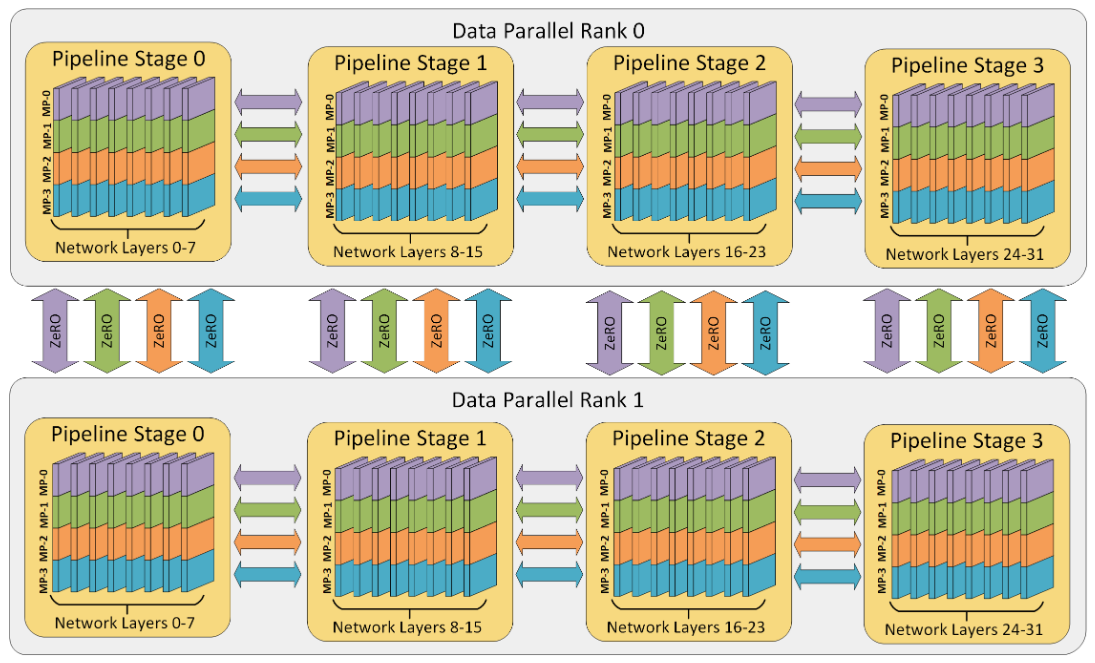
\includegraphics[scale=0.46]{Pipeline_Parallelism.png}}
	\caption{An overview of Pipeline Parallelism}
	\label{fig}
\end{figure*}

The first part of this project primarily focuses on Pipeline Parallelism, an approach that efficiently partitions model layers into various stages across the available accelerator devices. Furthermore, the internal working of each hardware accelerator is pipelined efficiently to improve peak memory usage and reduce communication costs across the worker nodes. Pipeline Parallelism is achieved using two general paradigms - synchronous gradient updates [1,3] (gradients are synced between adjacent training iterations to ensure convergence) and asynchronous gradient updates \cite{b2} (gradients stored locally to allow syncing later when needed). Using asynchronous gradient updates significantly increases memory footprint while also not ensuring convergence. Several recently developed libraries combine data and pipeline parallelism approaches to create an optimal pipeline. In particular, we look at systems employing hybrid parallelism (data and pipeline parallelism) with synchronous gradient update schemes. \\

GPipe's approach \cite{b1} to hybrid parallelism includes splitting a mini-batch of data into micro-batches and a model's layers into groups (stages) injected into the pipeline concurrently. The gradient updates are done synchronously and applied for each mini-batch. Even though this system improves device utilization and reduces communication overhead, it has several limitations. The forward activations must be stored for all micro-batches until the backward pass, increasing the memory footprint. This limitation is offset slightly by utilizing the re-computation strategy, which recomputes some of the activations of the forward pass at the expense of increased computation load.  \\
\begin{figure}[b]
	\centering
	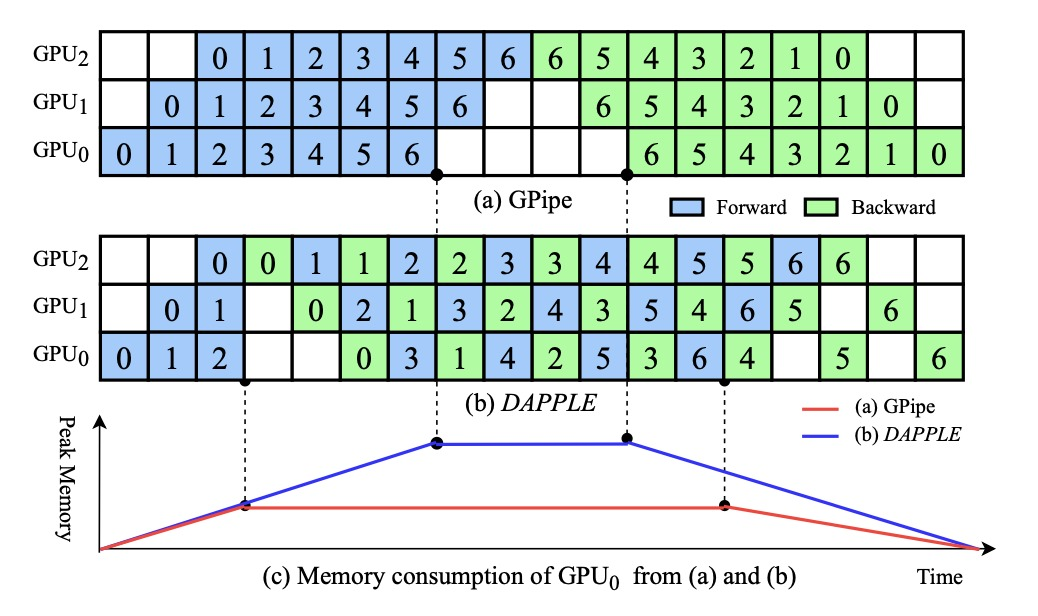
\includegraphics[scale=0.22]{GPipe_vs_DAPPLE.jpeg}
	\caption{GPipe vs DAPPLE: Scheduling Algorithms \cite{b4}}
	\label{fig}
\end{figure}

DAPPLE \cite{b4} strives to achieve better training convergence and memory efficiency using a hybrid parallelism method. The system consists of a Profiler stage (takes model layers as input and profiles execution time, activation, and parameter sizes for each layer), a Planner stage, and a Runtime stage. With the profiler's inputs, the planner handles the stage partition, stage replication, and device assignment to generate optimal parallelization plans. The device assignment algorithm is topology-aware and considers a broader solution space by considering three policies: Fresh First, Append First, and Scatter First. An important improvement of DAPPLE over GPipe is that instead of re-computation, the scheduler uses early backward scheduling to improve memory efficiency. Instead of injecting all micro-batches at once, a smaller number is injected first, and one forward pass of a micro-batch is interleaved with one backward pass. This interleaving approach relieves the memory pressure later on while maintaining high pipeline efficiency. This system significantly improved over GPipe regarding training throughput and memory consumption. \\

Harmony \cite{b5} also employs a hybrid parallelism method with improvements in the scheduling algorithm. It comprises three implementation stages - a Decomposer stage, which constructs a layer graph enabling each layer to be executed individually; a Profiler stage which records profiles (compute time, memory footprint, and input tensor size); and a Scheduler stage which uses the profiles and searches through the space of training configurations to find an optimal configuration to be run by the runtime. The profiler optimizes on two fronts - layer sizes and micro-batch sizes. Also, unlike GPipe and DAPPLE, where one stage is bound to one GPU, in Harmony, each GPU executes different forward and backward layer stages, which is enforced by a deterministic wrap-around schedule, a technique called wrap-around pipelining. Harmony has significantly improved training throughput and memory footprint during model training using these optimizations. \\

As an extension to studying synchronous Pipeline Parallelism techniques for training, we extend similar ideas for building distributed Model Inference techniques. We primarily evaluate two inference optimization libraries: Open Neural Network Exchange (ONNX) Runtime \cite{b6}, and DeepSpeed \cite{b7}. ONNX Runtime provides a high-performance inference engine for deploying models built using popular frameworks such as TensorFlow and PyTorch. Its runtime can build efficient Inference pipelines to leverage access to multi-accelerator environments. \\

DeepSpeed proposes a new approach for building efficient Inference pipelines based on Pipeline Parallelism-based techniques, emphasizing maximizing throughput and minimizing latency. DeepSpeed is focused on a specialized Inference Pipeline Parallelism approach which is further split into three stages: Scheduling, Memory Footprint Reduction, and Communication Optimization.


\section{Methodology}
\subsection{Proposed Solution and Implementation Details}
The initial stage of our solution mechanism will be to set up an evaluation baseline on existing Model Parallelism approaches for our designated tasks. This will also give us a good idea for developing implementation structures of commonly-used Parallelism techniques, post which we will transition to the synchronous Pipeline Parallelism approaches. \\

\subsubsection{Pipeline Parallelism for Model Training Tasks} 
The first synchronous pipeline parallelism approach for comparison is GPipe \cite{b1}, which consists of a torch-level implementation named torchgpipe \cite{b3}. GPipe is the first working algorithm that introduces an efficient synchronous pipeline parallelism scheme using micro-batching and memory re-materialization techniques. For our implementation, we first implemented torchgpipe for a simple image classification task built on the LeNet5 model for classifying the MNIST Dataset. We further extended this implementation for our primary Image Classification tasks (detailed in Section IV.C). One challenge for effectively deploying torchgpipe (primarily built on PyTorch) was to create Torch models using the Sequential Class. This proved to be quite a challenge, especially in building more complex models with unique layering concepts. 

The second approach for comparison is DAPPLE \cite{b4}, which follows implementation strategies similar to GPipe but also includes an early backward scheduling algorithm to find further exploitations in memory usage. As stated in the Literature Survey, DAPPLE is split into three key stages and is available as a Python library named HPGO. However, we were unable to the DAPPLE library completely across its end-to-end pipeline due to significant challenges in matching the required dependency versions. Although we extensively went through the underlying codebase for DAPPLE, we could not find any detail regarding the required dependency versions and hence, we omit publishing any concrete results for DAPPLE. However, we were able to successfully run the Profiler stage for DAPPLE which resulted in a clear text document containing layer-by-layer profiling details for any input CNN Model.

The third approach for comparison is Harmony \cite{b5}, which uses a customized scheduler that empirically evaluates the iteration time of each possible GPU configuration and automatically picks the best. For Harmony, we extensively test each stage of execution (as presented in the Literature Survey) and conclusively generate a viable end-to-end model specifically for Image Classification tasks. \\ 

\subsubsection{Pipeline Parallelism for Model Inference Tasks} 
During the Project proposal stage, our vision was to effectively combine various aspects of the aforementioned approaches to create an efficient Pipeline Parallelism algorithm for DNN Training. However, the introduction of large-scale Model Inference systems in our course material inspired us to investigate how complex Pipeline Parallelism approaches translate from Training to Inference Tasks. Hence, we further created a comparative study on two popular distributed Model Inference Solutions for Machine Translation Tasks. 

ONNX Runtime can accelerate the model inference time on NVIDIA GPUs for transformer models with a one-line addition for existing PyTorch training scripts. The use of the ONNX format for model inference enables developers to create and deploy machine learning models more easily and efficiently, with the flexibility to use different frameworks and target a variety of environments.

With ONNX, we compare DeepSpeed Inference, a full system solution for transformer model inference. When both dense and sparse transformer models fit in aggregate GPU memory, DeepSpeed Inference consists of a multi-GPU inference solution to minimize latency and maximize throughput, and when the full models cannot fit into a GPU a heterogeneous inference solution is implemented that makes use of CPU and NVMe memory in addition to GPU memory and compute to enable high inference throughput.

\subsection{Environment Setup}
For the bulk of our experiments, we trained and deployed models using Google Cloud Platform's (GCP) Compute Engine. We were able to acquire a maximum of 2 NVIDIA T4 GPUs with a 16GB Memory cap. We deployed instances with 2 Intel Xeon Microprocessors (2GHz frequency) each with 16GB RAM. In total, we spent a total of \$600 available as free starter credit. \\
Preliminary experiments were built using free credit GPU availability in Google CoLab. Each of our experiment setups featured several CUDA-assisted GPU Memory Profilers such as nvprof and nvidia-smi, including a few in-built code metrics to effectively calculate each implementation's throughput. For this project, we used CUDA v11.6.s

\begin{figure*}[t]
	\centering
	\fbox{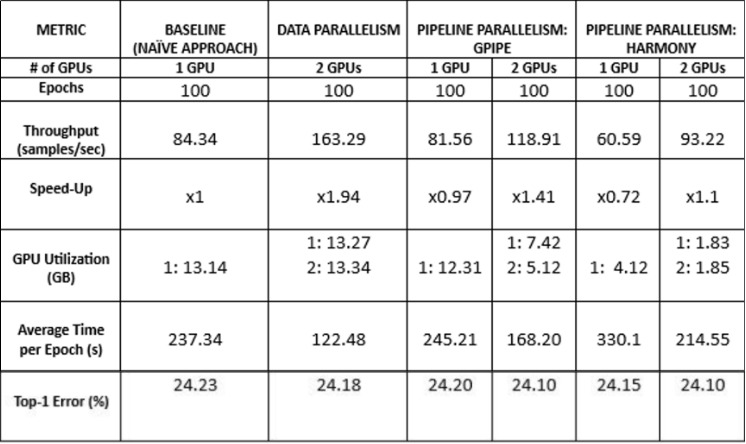
\includegraphics[scale=0.4]{Combined_Res.jpg}}
	\caption{Results for Pipeline Parallelism Techniques - Image Classification (Training) Task}
	\label{fig}
\end{figure*}

\subsection{Deep Learning Tasks}
\subsubsection{Image Classification for Model Training Tasks}
This project's scope will cover using Parallelism techniques for Image Classification tasks. Specifically, the project will use the ResNet50 Convolutional Neural Network model, an ideal choice for our experiments given that we are restricted to computational resources (GPUs). The ResNet50 model will be trained and evaluated on the ImageNet dataset. A naive implementation of ImageNet classification using ResNet50 (without parallelism techniques) will also provide a baseline for further experiments. For the scope of our project, it was not feasible for us to repeatedly test on the complete ImageNet dataset, owing to the dataset's very large size and lack of computation resources on our end. Hence, we developed our very own script to download any subset of ImageNet of our choice. We found it viable to create an ImageNet-based dataset with 100 unique classes and 200 images per class. This formed the universal dataset for each of our Model Training tasks.

\subsubsection{Machine Translation for Model Inference Tasks}
For benchmarking GPU-based inference models, we conducted experiments with the t5-small transformer model and the machine translation task. We used the main dataset of Workshop on Statistical Machine Translation (WML) 2015 from which we extracted 1000 samples of English to French translations for this project.


\subsection{Evaluation Metrics}
The following are the evaluation metrics designated to be used for the comparative analysis in this project:
\begin{enumerate}
    \item \textit{CPU / GPU memory utilization:} The goal is to maximize each worker node's CPU \& GPU efficiency (profiled using nvprof and nvidia-smi).
    \item \textit{Throughput:} The goal is to maximize the system's overall throughput (Data processing rate).
    \item \textit{Average time per epoch}: The goal is the minimize the system's average time per epoch.
    \item \textit{Top-1 Error Percentage (\%)}: The goal is to minimize the top-1 error percentage, i.e., maximize overall accuracy.
\end{enumerate}

\section{Evaluation Results}
\begin{figure}[h]
	\centering
	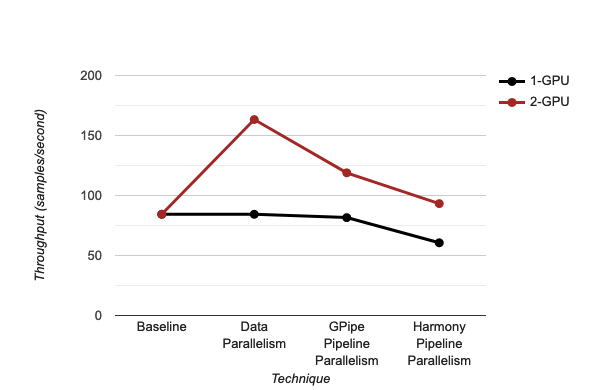
\includegraphics[scale=0.42]{FinalResultGraph.png}
	\caption{System Throughput Comparison - Image Classification (Training) Task}
	\label{fig}
\end{figure}
\subsection{Results for Training Tasks}
The results of the Image Classification-based Training Task are presented in Figure 3. Based on our findings, we find an interesting metric in which the 1-GPU Pipeline Parallelism models slightly underperform compared to the Naive implementation. With respect to GPipe, we attribute this slight drop-off to GPipe's requirement to recompute certain forward gradients during the backward pass. Concerning Harmony, we attribute the drop-off for Harmony to its inherent properties of being viable for multi-GPU settings only. We see that the 2-GPU Pipeline Parallelism models perform significantly better with respect to the baseline in terms of overall throughput, memory utilization, and accuracy. \\

The interesting analysis is the comparison between Pipeline Parallelism and Data Parallelism. It is straightforward to see that Data Parallelism provides the best throughput, as each available GPU is initialized with the complete model and not model splits, as is the case in Pipeline Parallelism. However, our approach for Data Parallelism does not fit into our GPU memory constraints even for the next iteration of the ResNet model series, i.e., ResNet-101. With this in mind, the GPU Utilization for our Pipeline Parallelism approaches is much superior to Data Parallelism. \\
Regarding the overall GPU memory footprint, we witness that the more elaborate memory-planning procedure followed in Harmony leads to a significant improvement to GPipe, with a trade-off in overall system throughput. \\
With respect to accuracy, we see that the Pipeline Parallelism approach holds a slight edge in comparison to the other systems. Figure 4 presents a graph that effectively compares the overall throughput of each implemented system.

\subsection{Results for Inference Tasks}
\begin{figure}[t]
	\centering
	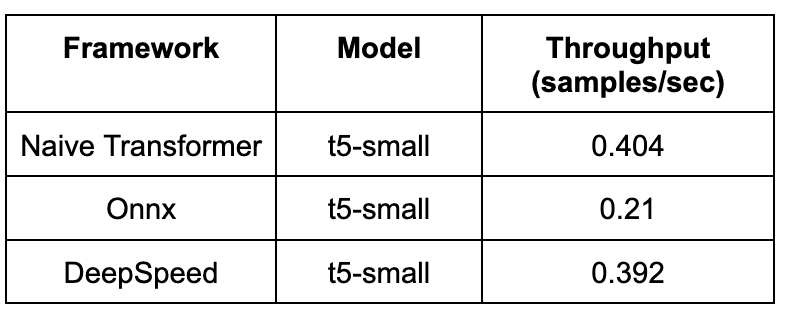
\includegraphics[scale=0.42]{Screenshots/Inference_Pic.png}
	\caption{Overall Results - Machine Translation (Inference) Task}
	\label{fig}
\end{figure}

We conducted experiments with the t5-small transformer model and the machine translation task to benchmark GPU-based inference models. The dataset consists of 1000 samples of English to French translations. We performed these experiments using the Google Cloud Platform's NVIDIA T4 GPUs. 
As expected, the naive transformer-based models performed the worst. But Onnx performs almost twice as fast as the naive transformer models. But surprisingly, DeepSpeed performs only slightly better than the naive model. This is because DeepSpeed has been specifically designed to use multiple GPUs and in cases where the entire machine-learning model cannot fit into memory. Since we were using the same transformer for all the implementations there was not any considerable difference in accuracy. The results are detailed in Figure 5.


\section{Conclusions and Key Learnings}
In this work, we have conducted several experiments on building efficient Pipeline Parallelism-based systems pertinent to DNN Model Training and Inference. \\
For Model Training, we observe that GPipe and Harmony provide unique and effective Pipeline Parallelism approaches. GPipe is efficient for maximizing throughput, and Harmony is efficient for reducing the overall memory footprint of the system. For Model Inference, ONNX presents significant scale-up opportunities in comparison to existing work. DeepSpeed also presents an efficient approach for building accurate inference systems for very large DNNs. \\
Based on our current implementations, we can further improve the efficacy of the approaches presented in this work with more fine-tuning of our systems. We expect our approaches to scale for much larger DNN models and datasets with more computation resources. \\

The crucial learning throughout this project was understanding the sophistication required to create scalable training and inference systems for DNN models. We learned the basic technicalities of relatively novel parallelism techniques crucial to building robust ML backends for the future. We also learned how to effectively profile hardware accelerator usage during DNN Training and Inference stages. Another key learning from working on a Machine Learning Systems project was patience's importance. We were put forth with getting available but complex codebases to work. Patience was important to maximize our learning and implement most of what we set out to do initially. \\
Furthermore, cloud GPUs are expensive, and a lengthy manual process is involved in assigning these GPUs to use. That hindered our progress since we had to share the available GPUs for all our model training, and we could not benchmark our project for more than 2 GPU usages.

\section{Future Work}
With an in-depth understanding of the implementation of synchronous Pipeline Parallelism for Model Training and Inference tasks, one immediate future work would be to extend our findings for much larger DNN models and datasets with larger hardware-accelerator capabilities (4-GPU and 8-GPU settings). \\
Another possible supplement to our work would be further fine-tuning our current DNN Training procedures implementations. For example, we can evaluate the ideal micro-batch size for different use cases. We can also compare our approaches to various asynchronous pipeline parallelism approaches such as PipeDream. \\
All in all, we firmly believe the primary future work of this project would be to formally define a single Pipeline Parallelism strategy that will increase the efficacy of both Training and Inference algorithms at the same time, which can further extend to building a single end-to-end pipeline incorporating ideas for both major use cases to sustain very large deep neural networks.

\section{Acknowledgements}
First and foremost, we would like to extend our immense appreciation to our professor, Dr. Jia Zou, who has played an instrumental role in providing essential background teachings and reference reading materials which had a tremendous impact in driving our interest and efforts pertaining to this project. We further extend our gratitude to the authors of our key references, who duly open-sourced their ideas to readily available frameworks, which streamlined our implementation and evaluation process.

\begin{thebibliography}{00}
\bibitem{b1} Yanping Huang et al, 2019. GPipe: Efficient training of giant neural networks using pipeline parallelism. Proceedings of the 33rd International Conference on Neural Information Processing Systems. Curran Associates Inc., Red Hook, NY, USA, Article 10, 103–112.
\bibitem{b2} Deepak Narayanan et al, 2019. PipeDream: generalized pipeline parallelism for DNN training. In Proceedings of the 27th ACM Symposium on Operating Systems Principles (SOSP '19). Association for Computing Machinery, New York, NY, USA, 1–15. https://doi.org/10.1145/3341301.3359646
\bibitem{b3} Kim, Chiheon, Heungsub Lee, Myungryong Jeong, Woonhyuk Baek, Boogeon Yoon, Ildoo Kim, Sungbin Lim and Sungwoong Kim. “torchgpipe: On-the-fly Pipeline Parallelism for Training Giant Models.” ArXiv abs/2004.09910 (2020): 
\bibitem{b4} Shiqing Fan et al, 2021. DAPPLE: a pipelined data parallel approach for training large models. In Proceedings of the 26th ACM SIGPLAN Symposium on Principles and Practice of Parallel Programming (PPoPP '21). Association for Computing Machinery, New York, NY, USA, 431–445. https://doi.org/10.1145/3437801.3441593
\bibitem{b5} Youjie Li et al, 2022. Harmony: overcoming the hurdles of GPU memory capacity to train massive DNN models on commodity servers. Proc. VLDB Endow. 15, 11 (July 2022), 2747–2760. https://doi.org/10.14778/3551793.3551828
\bibitem{b6} "ONNX Runtime", https://github.com/microsoft/onnxruntime
\bibitem{b7} Aminabadi, R. Y., Rajbhandari, S., Zhang, M., Awan, A. A., Li, C., Li, D., Zheng, E., Rasley, J., Smith, S., Ruwase, O., \& He, Y. (2022). DeepSpeed Inference: Enabling Efficient Inference of Transformer Models at Unprecedented Scale. ArXiv. /abs/2207.00032
\bibitem{b8} Oliver Rausch et al, 2022. A data-centric optimization framework for machine learning. In Proceedings of the 36th ACM International Conference on Supercomputing (ICS '22). Association for Computing Machinery, New York, NY, USA, Article 36, 1–13. https://doi.org/10.1145/3524059.3532364
\bibitem{b9} Juyong Kim et al, 2017. SplitNet: learning to semantically split deep networks for parameter reduction and model parallelization. In Proceedings of the 34th International Conference on Machine Learning - Volume 70 (ICML'17). JMLR.org, 1866–1874.
\bibitem{b10} Bian, Zhengda, Hongxin Liu, Boxiang Wang, Haichen Huang, Yongbin Li, Chuan-Qing Wang, Fan Cui and Yang You. “Colossal-AI: A Unified Deep Learning System For Large-Scale Parallel Training.” ArXiv abs/2110.14883 (2021)

\end{thebibliography} 

\end{document}